\documentclass[a4paper,12pt]{article} % тип документа

%  Русский язык
\usepackage[T2A]{fontenc}			% кодировка
\usepackage[utf8]{inputenc}			% кодировка исходного текста
\usepackage[english,russian]{babel}	% локализация и переносы

\usepackage{graphicx, scalerel}               % импорт изображений
\usepackage{wrapfig}                % обтекаемые изображения
\graphicspath{{pictures/}}          % обращение к подкаталогу с изображениями
\usepackage[14pt]{extsizes}         % для того чтобы задать нестандартный 14-ый размер шрифта
\usepackage[warn]{mathtext}         % русский язык в формулах
\usepackage{indentfirst}            % indent first
\usepackage[margin = 25mm]{geometry}% отступы полей
\usepackage[table,xcdraw]{xcolor}   % таблицы
\usepackage{amsmath,amsfonts,amssymb,amsthm,mathtools} % Математика
\usepackage{wasysym}                % ???
\usepackage{upgreek}                % ???  
\usepackage{caption}
\usepackage{multirow}
\captionsetup{labelsep=period}
\usepackage[font=small,labelfont=bf]{caption}
\usepackage{gensymb} % degree symbol
\usepackage{tikz}
\usetikzlibrary{positioning}


\begin{document}
	
	
	\begin{center}
		
		
		\textbf{НАЦИОНАЛЬНЫЙ ИССЛЕДОВАТЕЛЬСКИЙ УНИВЕРСИТЕТ \\ <<МОСКОВСКИЙ ФИЗИКО-ТЕХНИЧЕСКИЙ ИНСТИТУТ>>}
		\vspace{13ex}
		
		\textbf{Лабораторная работа 4.7.3\\ <<Изучение поляризованного света>>}
		\vspace{40ex}
		
		\normalsize{Овсянников Михаил Александрович \\ студент группы Б01-001\\ 2 курс ФРКТ\\}
	\end{center}
	
	\vfill 
	
	\begin{center}
		г. Долгопрудный\\ 
		2022 г.
	\end{center}
	
	
	\thispagestyle{empty} % выключаем отображение номера для этой страницы
	\newpage
	
	
	\textbf{Цель работы:} ознакомление с методами получения и анализа поляризованного света.
	
	\textbf{В работе используются:} оптическая скамья с осветителем; зеленый светофильтр; два поляроида; черное зеркало; полированная эбонитовая пластинка; стопа стеклянных пластинок; слюдяные пластинки разной толщины; пластинки в 1/4 и 1/2 длины волны; пластинка в одну длину волны для зеленого света (пластинка чувствительного оттенка).
	
	
	\section*{Теоретические сведения}
	\textbf{Естественный и поляризованный свет.} Как известно, световые волны поперечны: электрический вектор $\boldsymbol{E}$ и магнитный вектор $\boldsymbol{H}$ (или $\boldsymbol{B}$) взаимно перпендикулярны и располагаются в плоскости, перпендикулярной направлению распространения волны (лучу $\boldsymbol{S}$). Во всякой данной	точке пространства ориентация пары векторов $\boldsymbol{E}$ и $\boldsymbol{H}$ в плоскости, перпендикулярной лучу $\boldsymbol{S}$, может, вообще говоря, изменяться со временем. В зависимости от характера такого изменения различают естественный и поляризованный свет.
	\begin{figure}[h!]
		\centering
		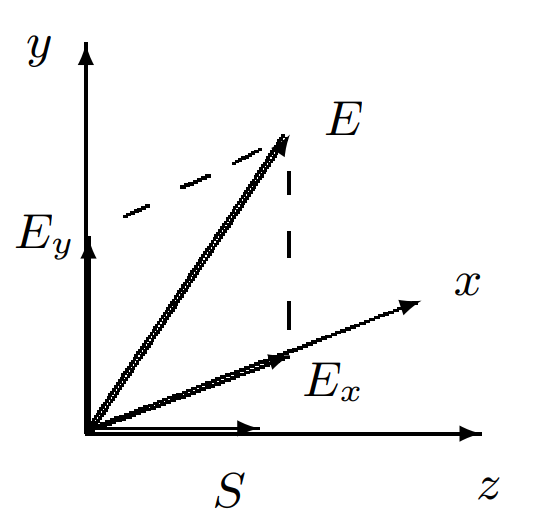
\includegraphics[scale=0.7]{Pictures/Decompose}
		\caption{Представление световой волны в виду двух линейно поляризованных волн}
	\end{figure}
	
	
	\textbf{Методы получения линейно поляризованного света.} Для получения линейно поляризованного света применяются специальные оптические приспособления — поляризаторы. Направление колебаний электрического вектора в волне, прошедшей через поляризатор, называется разрешенным направлением поляризатора. 
	
	Всякий поляризатор может быть использован для исследования поляризованного света, т. е. в качестве анализатора. Интенсивность $I$ линейно поляризованного света после прохождения через анализатор зависит от угла, образованного плоскостью колебаний с разрешенным направлением анализатора по закону Малюса:
	\begin{equation*}
		I = I_0 \cos^2\alpha.
	\end{equation*}


	Существует несколько способов получения плоскополяризованного света:
	\begin{enumerate}
		\item Отражение света от диэлектрической пластинки
		
		\item Преломление света в стеклянной пластинке
		
		\item Преломление света в двоякопреломляющих кристаллах
		
		\item Поглощение света в дихроических пластинках
	\end{enumerate}
	
	
	\textbf{Получение эллиптически поляризованного света.} Эллиптически поляризованный свет можно получить из линейно поляризованного с помощью двоякопреломляющих кристаллических пластинок. Например, пластинки $\lambda / 4$.

	
	\begin{figure}[h!]
		\begin{minipage}[h!]{0.49\linewidth}
			\center{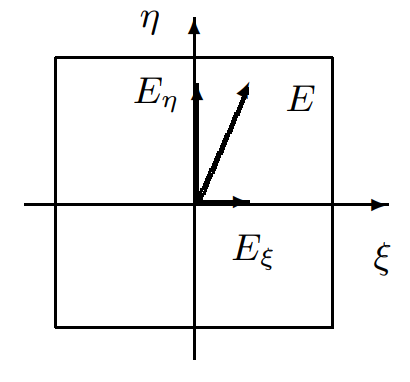
\includegraphics[width=\linewidth]{Pictures/EllipDecompose}} {а)}
		\end{minipage}
		\hfill
		\begin{minipage}[h!]{0.49\linewidth}
			\center{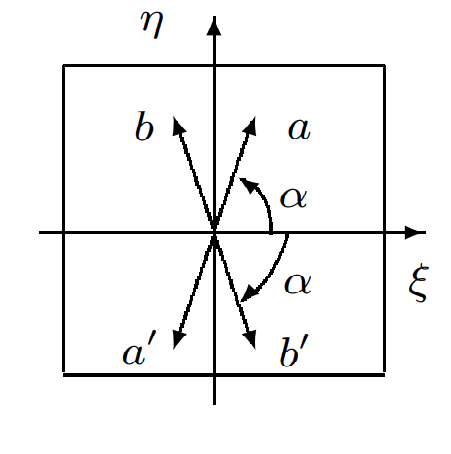
\includegraphics[width=\linewidth]{Pictures/LinFlip}} {б)}
		\end{minipage}
		\caption{a) Разложение линейно поляризованного света по главным направлениям двоякопреломляющей пластинки; б) Поворот направления колебаний с помощью пластинки в $\lambda/2$}
	\end{figure}	
		
	
	\textbf{Анализ эллиптически поляризованного света.} Анализ эллиптически поляризованного света сводится к нахождению главных осей эллипса поляризации и к определению направления вращения электрического вектора. Главные оси эллипса поляризации определяются с помощью анализатора по максимуму и минимуму интенсивности проходящего света.


	\textbf{Пластинка чувствительного оттенка.} Выше предполагалось известным, какому из двух главных направлений пластинки в четверть длины волны соответствует большая скорость распространения света. Установить это можно различными способами, например с помощью пластинки чувствительного оттенка (так называют пластинку в $\lambda$ для зеленой спектральной компоненты, $\lambda$ = 560 нм).	
	
	Пластинка имеет форму стрелы, вдоль оси которой расположено главное направление, соответствующее большей скорости распространения.
	
	\begin{wrapfigure}{r}{0.4\textwidth}
		\centering
		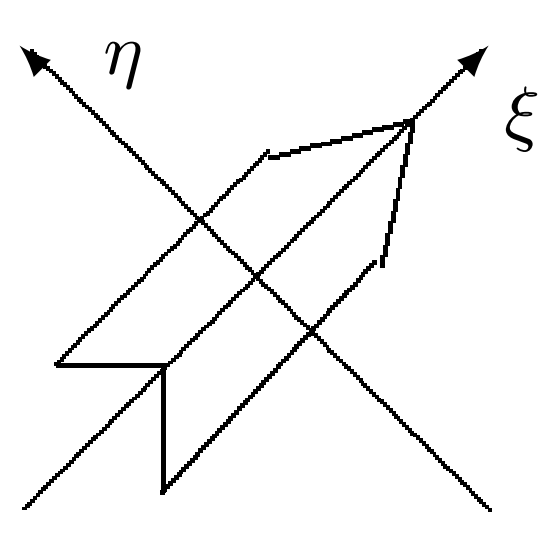
\includegraphics[scale=0.4]{Pictures/SensitivePlate}
		\caption{Пластинка чувствительного оттенка}
	\end{wrapfigure}
	
	Если пластинка чувствительного оттенка помещена между скрещенными поляроидами и главные направления пластинки не параллельны направлениям разрешенных колебаний поляроидов, то при освещении белым светом пластинка кажется окрашенной в лилово-красный цвет.
	
	Если между скрещенными поляроидами поместить пластинку чувствительного оттенка ($\lambda$) и пластинку в $\lambda$/4 так, чтобы их главные направления совпадали, цвет пластинки изменится.
	
	Если у пластинки чувствительного оттенка и пластинки в $\lambda$/4 совпадут главные направления, соответствующие большей скорости распространения, то разность хода между $E_{\xi}$ и $E_{\eta}$ для зеленого света составит уже 5$\lambda$/4. Это соответствует разности хода в $\lambda$ для света с большей длиной волны, т. е. для «более красного» света. При освещении этих пластинок белым светом теперь погасится не зеленая, а красная часть спектра, и проходящий свет будет казаться зеленовато-голубым. Если же главные направления, соответствующие большей скорости распространения, у пластинки чувствительного оттенка и у пластинки в $\lambda$/4 окажутся перпендикулярными, то проходящий свет приобретет оранжево-желтую окраску (погасится фиолетово-голубая часть спектра).
	
	\textbf{Интерференция поляризованных лучей.} Тонкие двоякопреломляющие пластинки, помещенные между поляроидами, кажутся окрашенными. Эта окраска может быть истолкована как результат интерференции поляризованных лучей.
	\begin{figure}[h!]
		\centering
		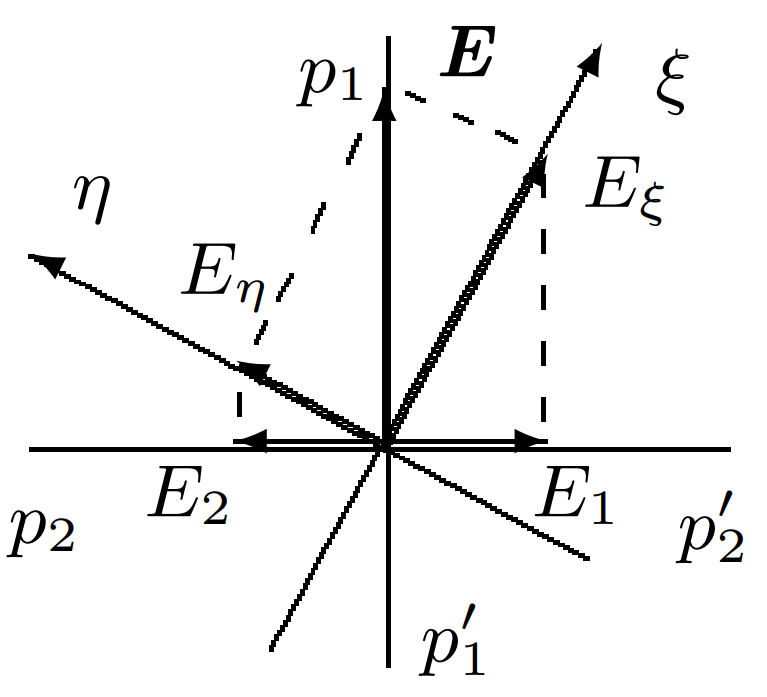
\includegraphics[scale=0.5]{Pictures/Interference}
		\caption{Объяснение интерференции поляризованного света}
	\end{figure}

	Здесь $p_1 p_1'$ — разрешенное направление колебаний поляризатора (первого поляроида); $\xi$, $\eta$ — координатная система, связанная с главными направлениями двоякопреломляющей пластинки; $p_2 p_2'$ — разрешенное направление колебаний анализатора (второго поляроида). Волны $E_\xi$ и $E_\eta$ на выходе из пластинки когерентны, но не могут интерферировать, так как $\boldsymbol{E}_\xi \perp \boldsymbol{E}_\eta$ Волны $E_1$ и $E_2$ на выходе второго поляроида также являются когерентными и к тому же поляризованы в одной плоскости. Эти волны интерферируют между собой. Результат интерференции определяется зависящим от длины волны сдвигом фаз между $E_1$ и $E_2$. В результате интерференции поляризованных лучей пластинка, освещаемая белым светом, кажется окрашенной.
	
	
	Если поворачивать двоякопреломляющую пластинку, расположенную между скрещенными поляроидами, то соотношение амплитуд волн $E_1$ и $E_2$ и разность фаз между ними не изменяются. Это означает, что цвет пластинки при ее поворотах не меняется, а меняется только интенсивность света. За один оборот пластинки интенсивность четыре раза обращается в нуль, — это происходит при совпадении главных направлений $\xi$ и $\eta$ с разрешенными направлениями колебаний поляроидов.
	
	Если же двоякопреломляющую пластинку оставить неподвижной, а второй поляроид повернуть так, чтобы разрешенные направления $p_1 p_1'$ и $p_2 p_2'$ совпали, то волны $E_1$ и $E_2$ приобретают дополнительный фазовый сдвиг на $\pi$ для всех спектральных компонент; поэтому цвет пластинки изменится на дополнительный.
	
	\newpage
	\section*{Ход работы}
	
	\begin{center}
		\textbf{I. Определение разрешённых направлений поляроидов}
	\end{center}

	\begin{enumerate}
		\item Разместим на оптической скамье осветитель $S$, поляроид $P_1$ и чёрное зеркало (пластинку чёрного стекла) так, чтобы плоскость падения была горизонтальна.
		
		\begin{figure}[h!]
			\centering
			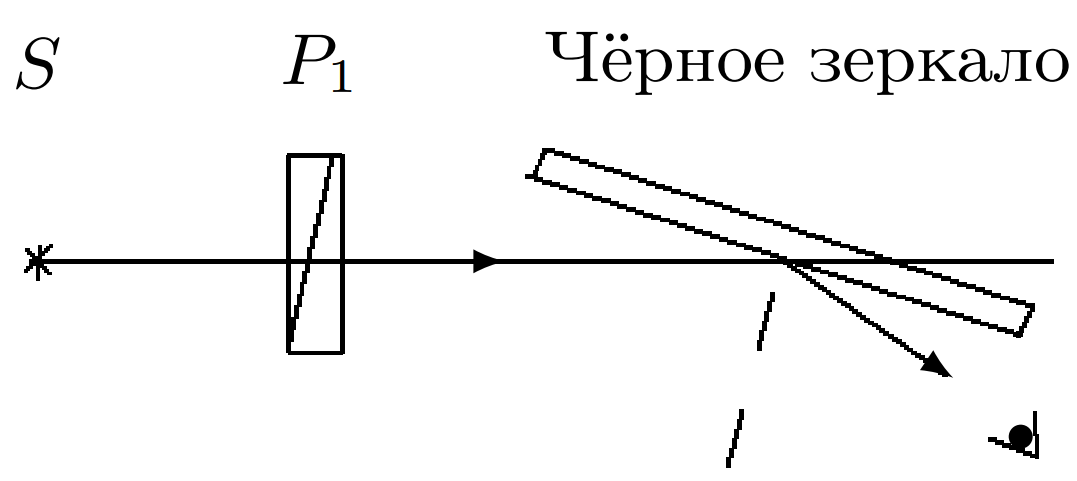
\includegraphics[scale=0.5]{Pictures/I}
			\caption{Определение разрешённого направления поляроида}
		\end{figure}
		
		\item Поворачивая поляроид вокруг направления луча, добьемся наименьшей яркости отражённого пятна. Оставим поляроид в этом положении и вращением зеркала вокруг вертикальной оси снова добьемся минимальной интенсивности отражённого луча. Уточним положения поляроида и зеркала, соответствующие минимуму интенсивности, и определим разрешённое направление поляроида:
		\begin{equation*}
			\boxed{\alpha_1 = (138\degree \pm 1\degree)}
		\end{equation*}
	
		\item Разрешённое направление второго поляроида можно определить, скрестив поляроиды: после поляроида с известной поляризацией поставим второй поляроид и, глядя навстречу лучу, вращением второго поляроида добьемся минимальной яркости луча:
		\begin{equation*}
			\boxed{\alpha_2 = (36\degree \pm 1\degree)}
		\end{equation*}
	\end{enumerate}


	\begin{center}
		\textbf{II. Определение угла Брюстера для эбонита}
	\end{center}

	\begin{enumerate}
		\item Поставим на скамью вместо чёрного зеркала эбонитовую пластину с круговой шкалой.
		
		\item Повернем эбонитовое зеркало вокруг вертикальной оси так, чтобы его плоскость была перпендикулярна лучу, и попытаемся совместить отражённое от эбонита пятно с отверстием осветителя. Отметим начало отсчёта по лимбу. Дальше все записи идут уже вычисленные относительно этого отсчета.
		
		\item Установим направление разрешённых колебаний поляроида $P_1$ горизонтально и найдем угол поворота эбонита $\varphi_{\text{Б}}$, при котором интенсивность отражённого луча минимальна:
		\begin{equation*}
			\boxed{\varphi_{\text{Б}} = (58\degree \pm 1\degree)}
		\end{equation*}
	
		Повторим измерения, добавив светофильтр Ф:
		\begin{equation*}
			\boxed{\varphi_{\text{Б}} = (57\degree \pm 1\degree)}
		\end{equation*}
		
		Нетрудно видеть, что эти два результата в пределах погрешностей совпадают.
	
		\item Теперь по найденному углу Брюстера рассчитаем показатель преломления эбонита $n = \tg\varphi_{\text{Б}}$.
		
		\textit{Без фильтра:} 
		\begin{equation*}
			\boxed{n = (1,60 \pm 0,06)}			
		\end{equation*}
		
		\textit{С фильтром:}
		\begin{equation*}
			\boxed{n = (1,54 \pm 0,06)}			
		\end{equation*}
	
		Видим, что опять же, в пределах погрешностей результаты совпадают. Причем, они даже совпадают с табличным значением $n = 1,6$. 
	\end{enumerate}	


	\begin{center}
		\textbf{III. Исследование стопы}
	\end{center}

	\begin{enumerate}
		\item Поставим стопу стеклянных пластинок вместо эбонитового зеркала и подберем для неё такое положение, при котором свет падает на стопу под углом Брюстера.
		
		\begin{figure}[h!]
			\centering
			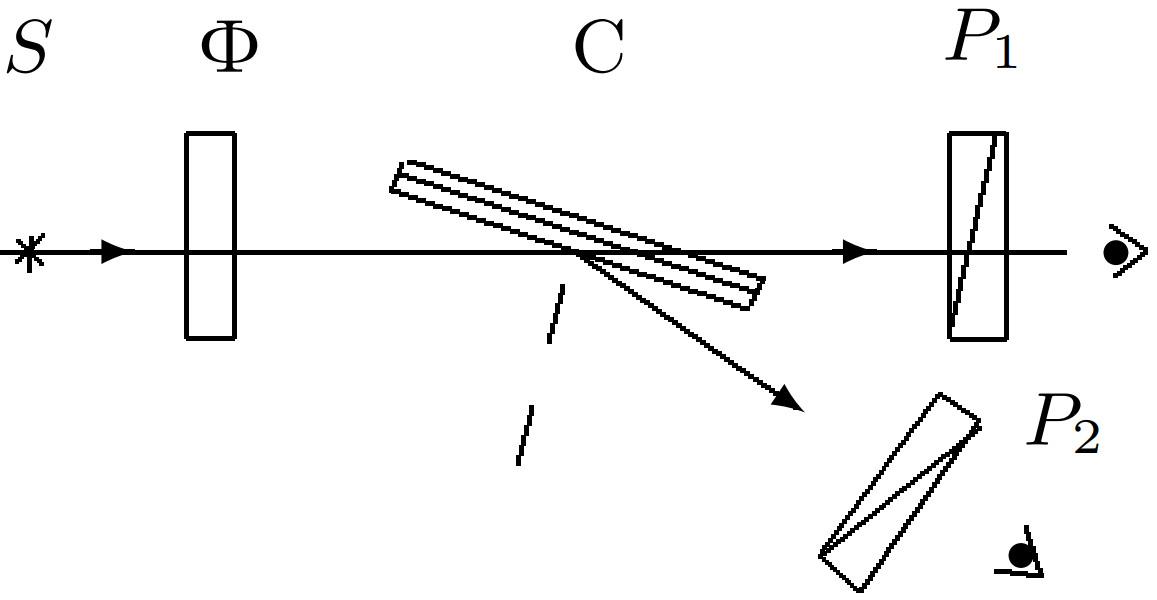
\includegraphics[scale=0.31]{Pictures/III}
			\caption{Исследование стопы}
		\end{figure}

		\item Осветим стопу неполяризованным светом (снимем поляризатор с оптической скамьи) и, рассматривая через поляроиды свет, отражённый от стопы, определим ориентацию вектора $\boldsymbol{E}$ в отражённом луче:
		
		$\bullet$ Поляризация линейная и угол $\alpha = 142\degree$ по поляризатору $P_1$.
		
		Теперь определим характер поляризации света в преломлённом луче:
		
		$\bullet$ Поляризация линейная и угол $\alpha = 55\degree$ по поляризатору $P_1$.
	\end{enumerate}

	\begin{center}
		\textbf{IV. Определение главных плоскостей двоякопреломляющих пластин}
	\end{center}

	\begin{enumerate}
		\item Поставим кристаллическую пластинку между скрещенными поляроидами $P_1$ и $P_2$.
		
		\begin{figure}[h!]
			\centering
			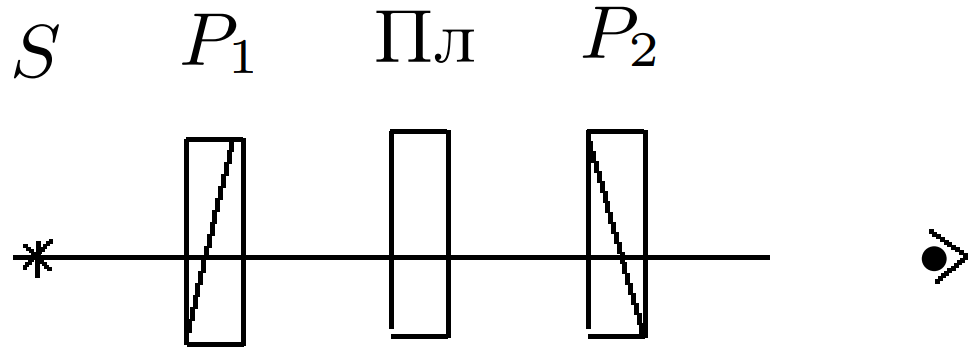
\includegraphics[scale=0.5]{Pictures/IV}
			\caption{Определение главных направлений в пластинках}
		\end{figure}
		
		\item Вращая пластинку вокруг направления луча и наблюдая за интенсивностью света, проходящего сквозь второй поляроид, определим, когда главные направления пластинки совпадают с разрешёнными направлениями поляроидов:
		
		\begin{center}
			$\bullet$ Минимумы первой пластинки: $26\degree$, $116\degree$, $206\degree$, $296\degree$.
		\end{center} 
		
		Повторим опыт для второй пластинки:
		
		\begin{center}
			$\bullet$ Минимумы второй пластинки: $14\degree$, $104\degree$, $194\degree$, $284\degree$.
		\end{center}
	\end{enumerate}


	\begin{center}
		\textbf{V. Выделение пластин $\lambda$/2 и $\lambda$/4}
	\end{center}

	\begin{enumerate}
		\item Добавим к предыдущей схеме зелёный фильтр; установим разрешённое направление поляроида горизонтально, а главные направления исследуемой пластинки — под углом $45\degree$ к горизонтали.
		
		\item С помощью второго поляроида установим, какую поляризацию имеет свет, прошедший пластинку: круговую или линейную с переходом в другой квадрант.
		
		У первой пластинки интенсивность не меняется с изменением угла, а значит, свет имеет круговую (эллиптическую)
		поляризацию. Таким образом, первая пластинка -- это $\lambda / 4$.
		
		\item Повторим то же для второй пластинки. Получаем, что при изменении угла второго поляроида свет имеет линейную поляризацию. Таким образом, вторая пластинка -- это $\lambda / 2$.
	\end{enumerate}


	\begin{center}
		\textbf{VI. Определение направлений большей и меньшей скорости в пластинке $\lambda$/4}
	\end{center}

	\begin{enumerate}
		\item Поставим между скрещенными поляроидами пластинку чувствительного оттенка ($\lambda$ для зелёного света), имеющую вид стрелки. Световой вектор, ориентированный вдоль направления стрелки, проходит с большей скоростью, перпендикулярный — с меньшей. Установим разрешённое направление первого поляроида горизонтально и убедимся с помощью второго поляроида, что эта пластинка не меняет поляризацию зелёного света в условиях предыдущего опыта.
		
		\begin{figure}[h!]
			\centering
			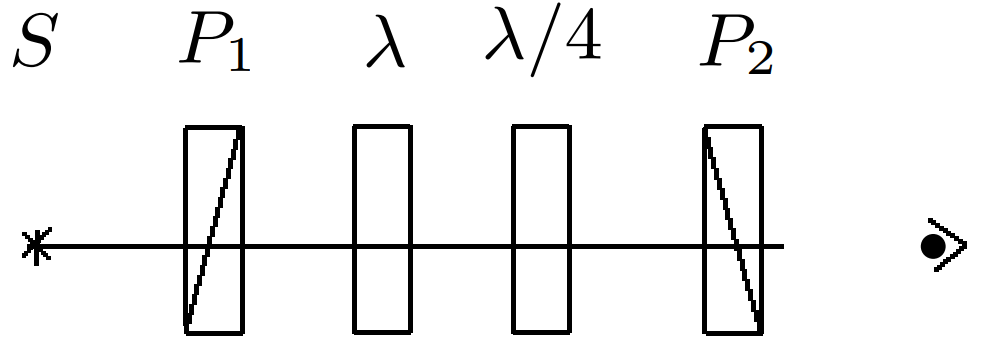
\includegraphics[scale=0.5]{Pictures/VI}
			\caption{Определение направлений большей и меньшей скорости}
		\end{figure}
		
		\item Уберем зелёный фильтр и поставим между скрещенными поляроидами пластинку $\lambda$. Глядя сквозь второй поляроид на стрелку, убедимся, что она имеет пурпурный цвет (зелёный свет задерживается вторым поляроидом, а красная и синяя компоненты проходят).
		
		\item Добавим к схеме пластинку $\lambda$/4, главные направления которой совпадают с главными направлениями пластины $\lambda$ и ориентированы под углом $45\degree$ к разрешённым направлениям скрещенных поляроидов. При повороте рейтера со стрелкой на $180\degree$ вокруг вертикальной оси цвет стрелки меняется от зелёно-голубого до оранжево-жёлтого. <<Быстрые оси>> совпадают, когда пластинка имеет зеленый цвет.
	\end{enumerate}

	
	\begin{center}
		\textbf{VII. Определение направления вращения светового вектора в эллиптически поляризованной волне}
	\end{center}

	\begin{enumerate}
		\item Нарисуем эллипс поляризации для вектора $\boldsymbol{E}$, вышедшего из пластинки $\lambda$/4, и укажем на нём направления большей и меньшей скорости. На рисунке $x$ -- большая скорость, а $y$ -- меньшая. Рядом нарисуем две вышедших из пластинки синусоиды: $x(t)$ и $y(t)$ со сдвигом фаз в четверть периода. По рисунку направление вращения электрического вектора в эллиптически поляризованной волне против часовой стрелки.
		
		\begin{figure}[h!]
			\begin{minipage}[h!]{0.49\linewidth}
				\center{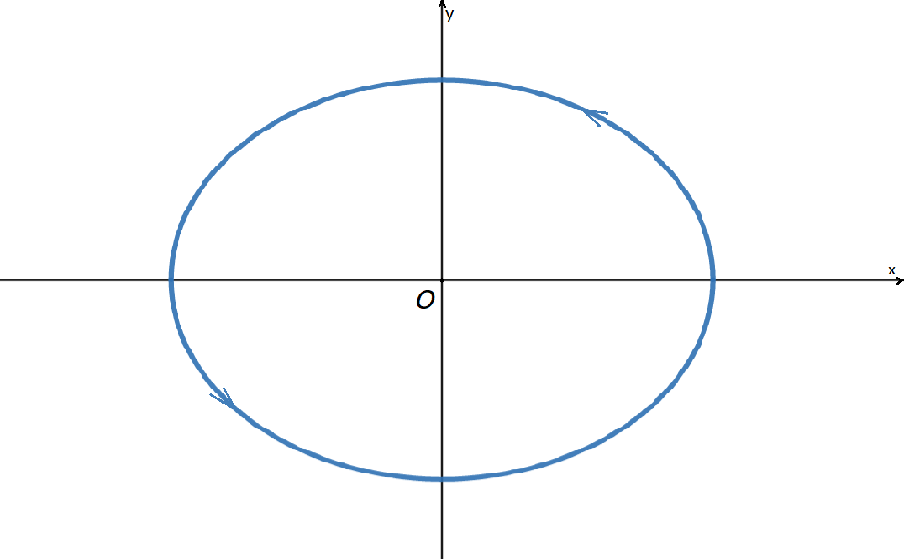
\includegraphics[width=\linewidth]{Pictures/Эллипс}}
			\end{minipage}
			\hfill
			\begin{minipage}[h!]{0.49\linewidth}
				\center{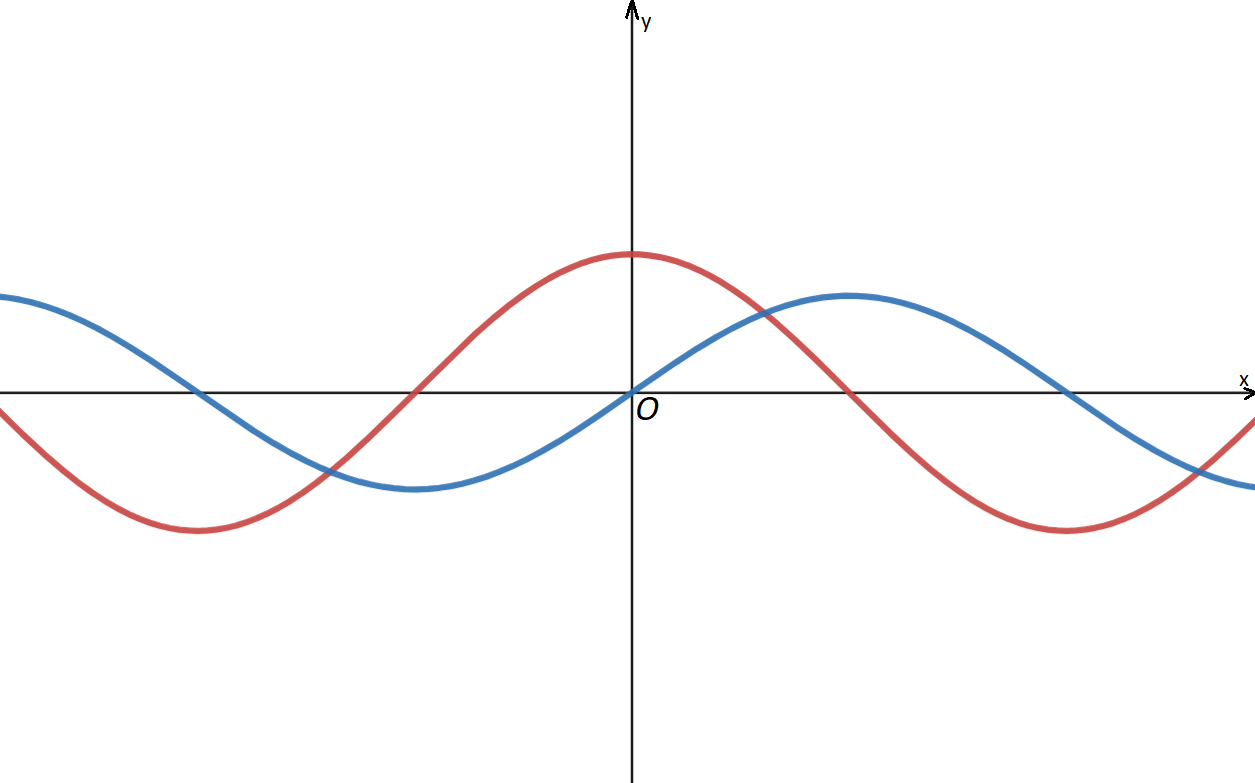
\includegraphics[width=\linewidth]{Pictures/Синусоиды}}
			\end{minipage}
			\caption{Эллипс поляризации и синусоиды}
		\end{figure}
	
	
		\item Снова поставим зелёный фильтр, а за ним между скрещенными поляроидами — пластинку $\lambda$/4 с соседней установки.
		
		\item Получим эллиптически-поляризованный свет. Для этого установим разрешённое направление первого поляроида под углом 10–20$\degree$ к горизонтали так, чтобы вектор $\boldsymbol{E}$ падающего на пластинку света был расположен в первом квадранте. Установим разрешённое направление второго поляроида вертикально и, вращая пластинку, найдем минимальную интенсивность света, прошедшего второй поляроид. Вращая второй поляроид, убеждаемся, что свет поляризован эллиптически, а не линейно. Таким образом, был получен эллипс поляризации с вертикально ориентированной малой осью.
		
		\item Для определения направления вращения светового вектора в эллипсе установим между поляроидами дополнительную пластинку $\lambda$/4 с известными направлениями «быстрой» и «медленной» осей, ориентированными по осям эллипса поляризации анализируемого света. В этом случае вектор $\boldsymbol{E}$ на выходе будет таким, как если бы свет прошёл две пластинки $\lambda$/4: свет на выходе из второй пластинки будет линейно поляризован. Если пластинки поодиночке дают эллипсы, вращающиеся в разные стороны, то поставленные друг за другом, они скомпенсируют разность фаз, и вектор $\boldsymbol{E}$ на выходе останется в первом и третьем квадрантах. Если же световой вектор перешёл в смежные квадранты, значит, эллипсы вращаются в одну сторону.
		
		По эксперименту получили, что эллипсы вращаются в одну сторону. Таким образом, световой вектор в эллиптически поляризованной волне имеет направление вращения против часовой стрелки.
	
	\end{enumerate}


	\begin{center}
		\textbf{VIII. Интерференция поляризованных лучей}
	\end{center}

	\begin{enumerate}
		\item Расположим между скрещенными поляроидами мозаичную слюдяную пластинку. Она собрана из 4-х узких полосок слюды, лежащих по сторонам квадрата (две полоски «толщиной» $\lambda$/4 и по одной — $\lambda$/2 и 3$\lambda$/4). Что-то похожее на это:
		
		\begin{figure}[h!]
			\centering
			\begin{tikzpicture}

				\draw (0, 0)    rectangle (1.5, 1.5) node[pos=0.5] {$\frac{3\lambda}{4}$};
				\draw (1.5, 0)  rectangle (3, 1.5)   node[pos=0.5] {$\lambda$};
				\draw (-1.5, 0) rectangle (0, 1.5)   node[pos=0.5] {$\lambda$};
				
				\draw (0, -1.5)    rectangle (1.5, 0) node[pos=0.5] {$0$};
				\draw (1.5, -1.5)  rectangle (3, 0)   node[pos=0.5] {$\frac{\lambda}{4}$};
				\draw (-1.5, -1.5) rectangle (0, 0)   node[pos=0.5] {$\frac{\lambda}{4}$};
			
				\draw (0, -3)    rectangle (1.5, -1.5) node[pos=0.5] {$\frac{\lambda}{2}$};
				\draw (1.5, -3)  rectangle (3, -1.5)   node[pos=0.5] {$\frac{3\lambda}{4}$};
				\draw (-1.5, -3) rectangle (0, -1.5)   node[pos=0.5] {$\frac{3\lambda}{4}$};
				
				\draw[blue, ultra thick] (-1.5, 0)  rectangle (3, 1.5);
				\draw[blue, ultra thick] (-1.5, -3) rectangle (3, -1.5);
				\draw[red,  ultra thick] (-1.5, -3) rectangle (0, 1.5);
				\draw[red,  ultra thick] (1.5, -3)  rectangle (3, 1.5);
				
				
				\draw [-latex] (-0.75, 2.75) -- (-0.75, 1.75);
				\node at (-0.75, 3.25) {$\frac{\lambda}{4}$};
				
				\draw [-latex] (2.25, 2.75) -- (2.25, 1.75);
				\node at (2.25, 3.25) {$\frac{\lambda}{4}$};
				
				\draw [-latex] (4.25, 0.75) -- (3.25, 0.75);
				\node at (4.75, 0.75) {$\frac{3\lambda}{4}$};
				
				\draw [-latex] (4.25, -2.25) -- (3.25, -2.25);
				\node at (4.75, -2.25) {$\frac{\lambda}{2}$};
				
			\end{tikzpicture}
			\caption{Мозаичная пластинка}
		\end{figure}
	
	\item В центральном квадратике слюды нет. Главные направления всех пластинок ориентированы параллельно сторонам квадрата.
	
	\item Вращая пластинку и второй поляроид будем наблюдать за изменениями интенсивности и цвета в отдельном квадратике.
	\end{enumerate}
	\textit{Вращаем пластинку:}
	\vspace{5mm}
	
	\noindent Центральный квадратик всегда черный. Это объясняется тем, что он не покрыт слюдой, а свет проходит через него и скрещенные поляроиды, поэтому интенсивность нулевая.
	
	\noindent Боковые квадратики изменяют как свой цвет, так и свою интенсивность. Периодичность $\frac{\pi}{4}$.
	\newpage

	\noindent \textit{Вращаем поляроид:}
	\vspace{5mm}
	
	\noindent Теперь и центральный квадратик изменяет интенсивность и цвет. Это потому, что теперь разрешенные направления поляроидов не являются скрещенными.
	
	\vspace{12cm}
	\section*{Вывод}
	В данной работе мы познакомились с методами получения поляризованного света и способами его анализа. Были определены разрешенные направления конкретных поляроидов, использованных в этой работе: $\alpha_1 = (138\degree \pm 1\degree)$ и $\alpha_2 = (36\degree \pm 1\degree)$. Был определен угол Брюстера для эбонита: $\varphi_{\text{Б}} = (58\degree \pm 2\degree)$, откуда был найден и показатель преломления: $n = (1,57 \pm 0,09)$. Была исследована стопа Столетова, определены главные плоскости двоякопреломляющих пластин, а также направления большей и меньшей скорости в пластинке в четверть длины волны. Мы пронаблюдали эллиптическую поляризацию и интерференцию поляризованных лучей. Хотя большинство экспериментов носило качественный характер, численные значения найденных величин имеют погрешности. Они связаны с неточностью измерений -- как минимум с неточностью выставления зеркала, стопы или пластин.

\end{document}